\newpage
\section{Дистрибуция пакетов в Windows}

В мире Windows распространение программ осуществляется при помощи инсталляционных пакетов.

Inno Setup -- система создания инсталляторов для Windows программ с открытым исходным кодом. Впервые выпущенный в 1997 году, отличается функциональности и стабильности. Кроме того, обладает интерфейсом, к которому привыкли многие пользователи.

Inno Setup графическим интерфейсом, который (по средствам мастера) позволяет создать скрипт, на основании которого генерируется установочный пакет. Скрипт для разрабатываемой программы netmonitor представлен в листинге 5.

\lstinputlisting[language={},caption={Скрипт генерации установочного файла}]{res/netmonitor.iss}

Получив установочный пакет, можно его распространять на других Windows-системах. Установка также происходит при помощи графического мастера и не должна вызывать сложности у пользователя (Рисунок 2).

\begin{figure}[H]
 \centering
 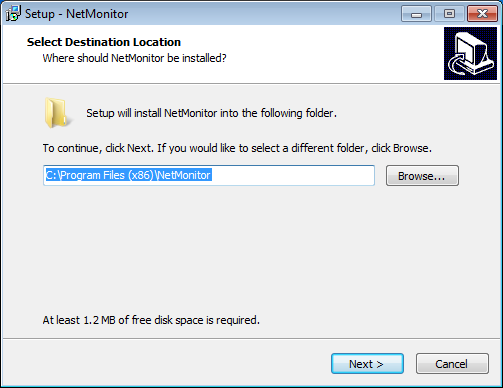
\includegraphics[scale=1]{res/pic002}
 \caption{Интерфейс установки приложения netmonitor}
\end{figure}